\documentclass[tikz,border=8pt]{standalone}
\usepackage[utf8]{inputenc}
\usepackage[OT4,plmath]{polski}
\usepackage{amsmath}
\usetikzlibrary{patterns}
\begin{document}
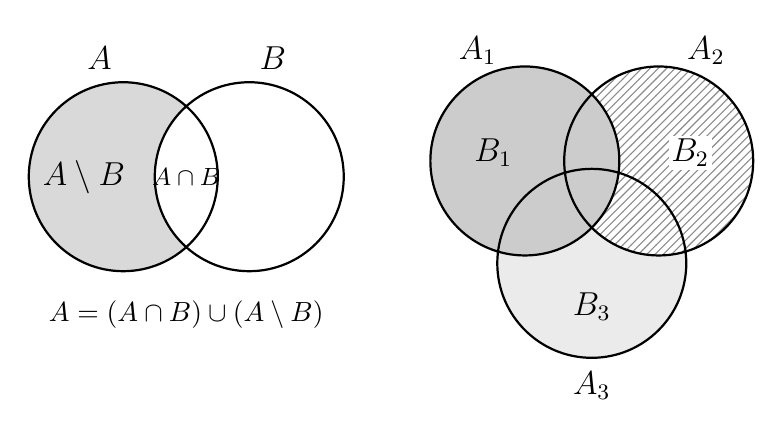
\begin{tikzpicture}[font=\large]
  \fill[black!15] (1.4,1.5) circle (1.2);
  \fill[white] (3,1.5) circle (1.2);
  \draw[thick] (1.4,1.5) circle (1.2) (3,1.5) circle (1.2);
  \node at (.9,1.5) {$A\setminus B$};
  \node[font=\small] at (2.2,1.5) {$A\cap B$};
  \node at (1.1,3) {$A$};
  \node at (3.3,3) {$B$};
  \node[font=\normalsize] at (2.2,-.25)
    {$A=(A\cap B)\cup(A\setminus B)$};

  \fill[black!20] (6.5,1.7) circle (1.2);
  \begin{scope}[even odd rule]
    \clip (8.2,1.7) circle (1.2);
    \clip (4,-1) rectangle (10,4) (6.5,1.7) circle (1.2);
    \fill[pattern=north east lines,pattern color=black!45] (4,-1) rectangle (10,4);
  \end{scope}
  \begin{scope}[even odd rule]
    \clip (7.35,.4) circle (1.2);
    \clip (4,-1) rectangle (10,4) (6.5,1.7) circle (1.2);
    \clip (4,-1) rectangle (10,4) (8.2,1.7) circle (1.2);
    \fill[black!8] (4,-1) rectangle (10,4);
  \end{scope}
  \draw[thick] (6.5,1.7) circle (1.2) (8.2,1.7) circle (1.2)
    (7.35,.4) circle (1.2);
  \node at (6.1,1.8) {$B_1$};
  \node[fill=white,inner sep=1pt] at (8.6,1.8) {$B_2$};
  \node at (7.35,-.15) {$B_3$};
  \node at (5.9,3.1) {$A_1$};
  \node at (8.8,3.1) {$A_2$};
  \node at (7.35,-1.15) {$A_3$};
\end{tikzpicture}
\end{document}
